\documentclass[12pt]{article}

\usepackage{float}
\usepackage{dsfont}
\usepackage{amsmath}
\usepackage{amsthm}
\usepackage{graphicx}

\usepackage[font=footnotesize,labelfont=bf]{caption}

\usepackage{bm}
\newcommand{\m}[1]{\mathbf{\bm{#1}}}
\newcommand{\R}{I\hspace{-4.4pt}R}

\begin{document}

\noindent AMS 263 --- Stochastic Processes

\noindent Mickey Warner
\bigskip

\begin{center}
\begin{large}
California precipitation extremes during 1950--1999
\end{large}
\end{center}

\section*{Introduction}

\subsection*{Precipitation data}

\noindent In this report we analyze the extreme behavior of daily total precipitation in California from 1950 through 1999. The data are taken from Ed Maurer's website at http://www.engr.scu.edu/$\sim$emaurer/data.shtml. Data are collected from various weather stations across the United States and then interpolated to obtain daily values on a fine grid (about $1/8^\circ$ spacing). Data are shown in Figure 1.

\begin{figure}[H]
\begin{center}
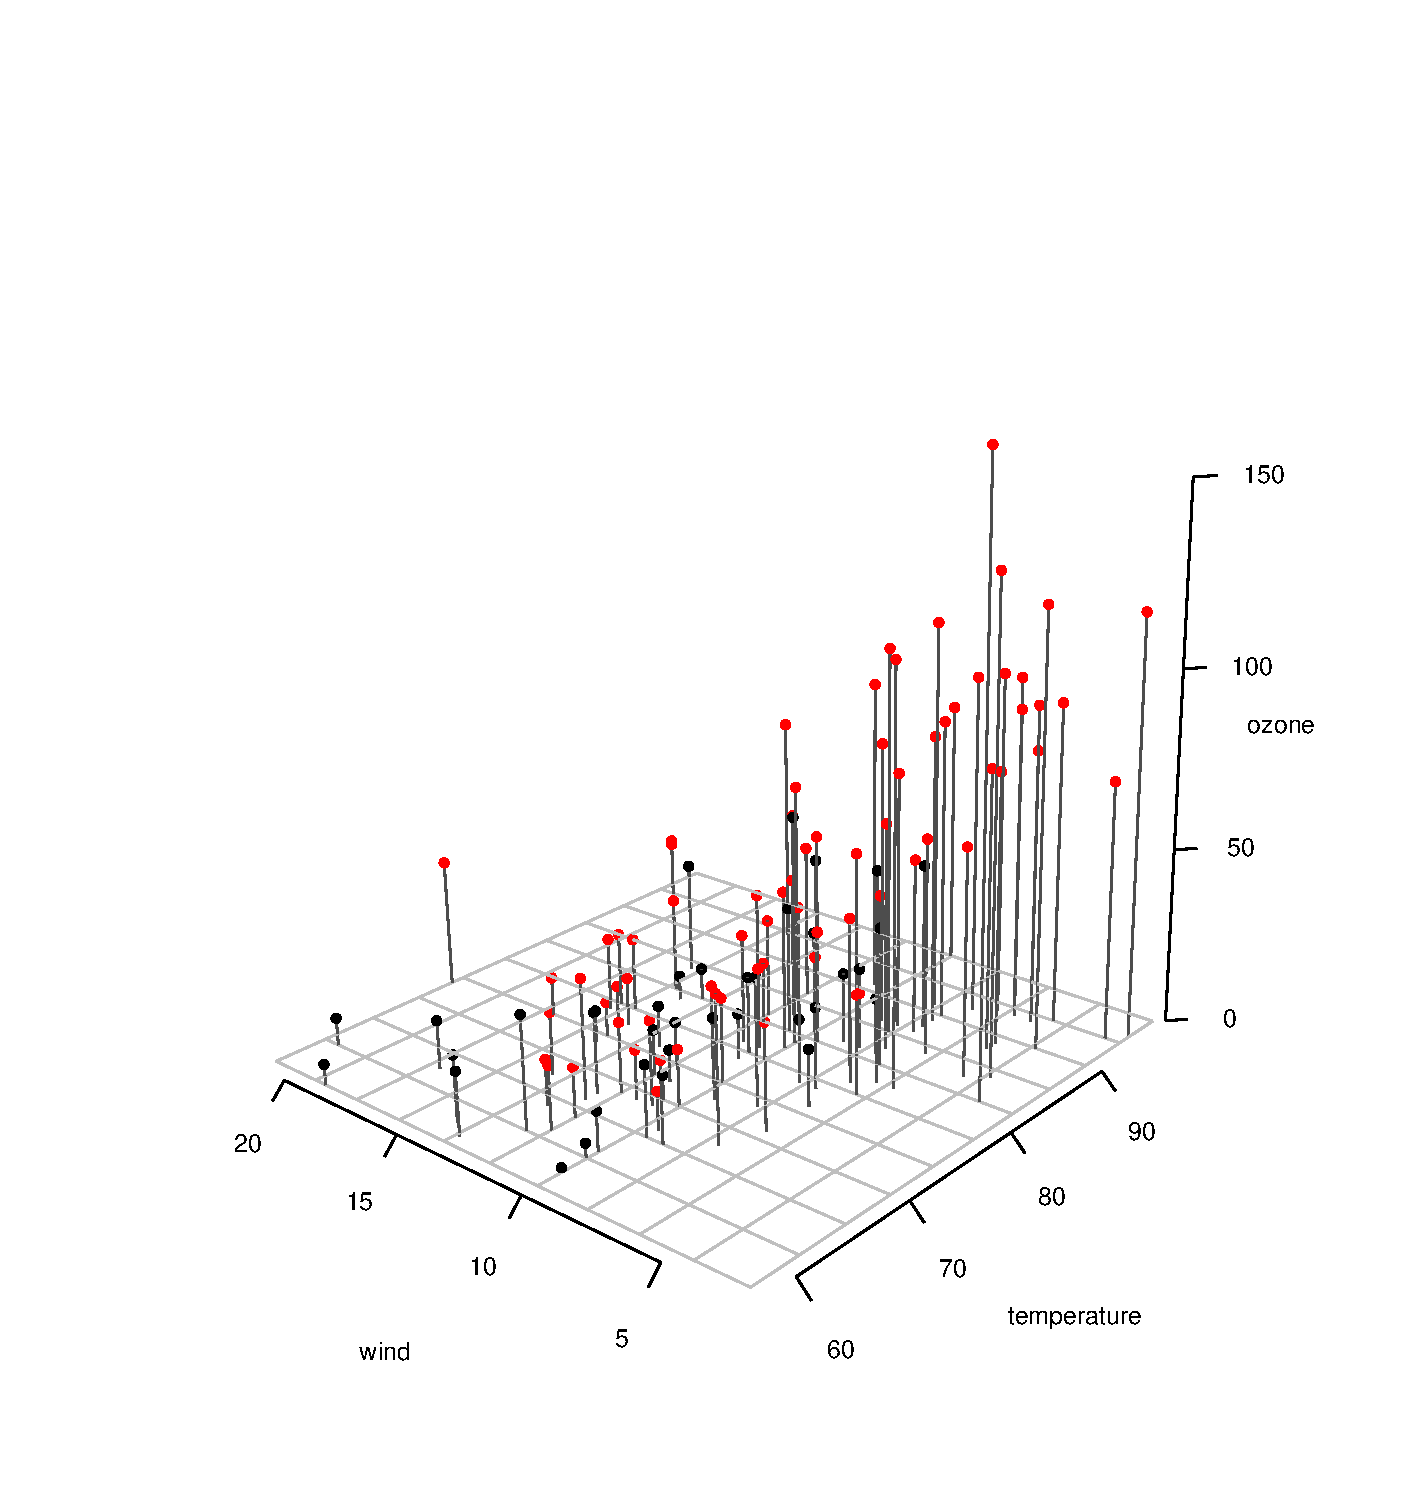
\includegraphics[scale=0.40]{../figs/data.pdf}
\end{center}
\caption{Daily total precipitation in California for the years 1950 through 1955.}
\end{figure}

\subsection*{Some extreme value theory}

\noindent Our goal is to characterize the extreme behavior in the process determining precipitation. Extreme value theory yields the following theorem relating large values of random variables and the Poisson process.
\bigskip

\noindent \textbf{Theorem.} Let $X_1,\ldots,X_n$ be a series of independent and identically distributed random variables, and let
\[ N_n = \{(i/(n+1), X_i):i=1,\ldots,n\}. \]
\noindent Then, for sufficiently large $u$, on regions of the form $(0,1)\times[u,\infty)$, $N_n$ is approximately a Poisson process with intensity measure on $A=[t_1,t_2]\times(z,\infty)$ given by
\[ \Lambda(A) = (t_2-t_1)\left[1+\xi\left(\frac{z-\mu}{\sigma}\right)\right]^{-1/\xi}. \]
\qed
\bigskip

\noindent For a given $u$, letting $A=(0,1)\times[u,\infty)$ and re-labeling the observations that fall in $A$ as $(t_1,x_1,\ldots,t_{N(A)},x_{N(A)})$, it can be shown that likelihood is given by
\[ L \propto \exp\left\{-n_y\left[1+\xi\left(\frac{u-\mu}{\sigma}\right)\right]^{-\frac{1}{\xi}}\right\}\prod_{i=1}^{N(A)}\frac{1}{\sigma}\left[1+\xi\left(\frac{x_i-\mu}{\sigma}\right)\right]^{-\frac{1}{\xi}-1} \]
\noindent where $n_y$ is the number of years of observation (here $n_y=50$), so that the parameters correspond to the annual maximum distribution.
\bigskip

\noindent The value $u$ is called the threshold and variables exceeding $u$ are called extreme. Care must be taken when selecting $u$: too low and the approximation to the Poisson process may be unreasonable, too high and there may be too few data points to obtain reasonable estimates for the parameters $(\mu, \sigma, \xi)$.
\bigskip

\noindent The most important parameter in an extreme value setting is $\xi$. $\xi$ describes the tail behavior. When $\xi<0$, there is an upper bound at $z^*=\mu-\sigma/\xi$. When $\xi\geq 0$, then the first $\lfloor{1/\xi-1}\rfloor$ moments exist. This means that when $\xi>1$, we have no moments, or a long right tail.

\section*{Methods}

\noindent The data shown in Figure 1 clearly exhibit a periodic pattern: unsurprisingly, we observe more precipitation in the winter months than we do in the summer months. This present at least two options. First, since the kind of precipitation levels we need to be concerned about (on a practical level) will be occurring during the winter, we could simply perform the analysis on the winter data only. In this case, we may expect independent and identically distributed random variables, a useful assumption.
\bigskip

\noindent The second option is to perform the analysis with time-varying aspects in the model. This is the approach we take here. As we will see, option one may be preferable, but I believe the second option can highlight some crucial (and perhaps unnecessary) difficulties with the time-varying model.

\subsection*{Threshold selection}

\noindent Our first task is to select a threshold that depends on time $u_t$. To do this, we take a ``moving quantile'' across the data points. We compute the $95\%$ quantile of the observations in a window of size $30$. We then fit a regression with annual and semi-annual periods on the log of the observed quantiles. Exponentiating the mean of the regression gives us our time-varying threshold, shown in blue in Figure 2.

\begin{figure}[H]
\begin{center}
\includegraphics[scale=0.30]{../figs/threshold.pdf}
\end{center}
\caption{California precipitation data with time-varying threshold.}
\end{figure}

\noindent A valid threshold for independent observations should yield exceedances that occur roughly uniformly across time. Figure 3 shows the frequency of exceedances by month and by year. Clearly, some years contribute the most in exceedances (1982, 1983, and 1998). 

\begin{figure}[H]
\begin{center}
\includegraphics[scale=0.30]{../figs/exceedance_loc.pdf}
\end{center}
\caption{Rate of exceedance by month (left) and year (right).}
\end{figure}

\subsection*{Parameter estimation}

\noindent We also assume that $\mu$, $\log \sigma$, and $\xi$ all have an annual cycle. For time $t$, we define $\mu_t = \beta_0 + \beta_1 \cos(2\pi/365*t) + \beta_2\sin(2\pi/365*t)$. Similar forms are assumed for $\log \sigma$ and $\xi$.
\bigskip

\noindent Normal(0, $100^2$) priors are placed on each of the coefficients for $\mu_t$, $\log \sigma_t$, and $\xi_t$. Posterior samples are easily obtained using standard MCMC algorithms.

\subsection*{Return levels}

\noindent Denoting $z_m$ to be the $m$-year return level, and letting $n$ be the number of observations in a year, $z_m$ satisifes the equation
\[ 1-\frac{1}{m}=\Pr\{\max(X_1,\ldots,X_n)\leq z_m\} \approx \prod_{i=1}^n p_i, \]
\noindent where $p_i=1-n^{-1}[1+\xi_i(z_m-\mu_i)/\sigma_i]_+^{-1/\xi_i}$. The value $z_m$ is interpreted as the level we expect to see the maximum exceed on average once every $m$ observations. When the process is stationary (as we might assume if we look at winter only data), then solving for $z_m$ is straightforward.
\bigskip

\noindent We can obtain posterior samples for $z_m$ in the non-stationary process by plugging in our posterior samples of $(\mu_i,\sigma_i,\xi_i)$ to $p_i$ and repeatedly solving for $z_m$. What we do here, however, is calculate the return level for a specific day in the year, thus solving for $z_m^{(t)}$ in
\[ 1 - \frac{1}{m} = \Pr(X_t \leq z_m^{(t)}) = 1 - [1 + \xi_t(z_m^{(t)}-\mu_t)/\sigma_t]^{-1/\xi_t},~~~~~t=1,\ldots,365 \]
\noindent for which posterior samples are easily obtained.

\section*{Results}

\noindent Posterior distributions over a one-year time spawn are shown in Figure 4. There appears to be some evidence that $\xi$ need not be explained with time-varying components, as a horizontal line can pass through between the lower and upper 95\% bounds. The estimates for $\mu$ seem to be counterintuitive. We expected to see that $\mu$ is greater in the winter months, suggesting perhaps that either our formulation for $\mu_t$ is invalid, or we have selected a poor choice of threshold $u_t$.

\begin{figure}[H]
\begin{center}
\includegraphics[scale=0.22]{../figs/post_mu.pdf}
\includegraphics[scale=0.22]{../figs/post_sig.pdf}
\includegraphics[scale=0.22]{../figs/post_ksi.pdf}
\end{center}
\caption{Posterior mean and 95\% credible bounds for $(\mu_t,\sigma_t,\xi_t)$, for $t=1,\ldots,365$. The vertical lines divide the region into months.}
\end{figure}

\begin{figure}[H]
\begin{center}
\includegraphics[scale=0.30]{../figs/return10.pdf}
\includegraphics[scale=0.30]{../figs/return20.pdf}
\includegraphics[scale=0.30]{../figs/return50.pdf}
\end{center}
\caption{Return levels for each day in the year. The black region in each plot denotes the 95\% return level. The colored dots are the 10 largest observations for that given day (across all years), ranging from red (10th largest) to purple (largest). A black line connects the largest observations at each day.}
\end{figure}

\noindent In Figure 5 we show the $10$-, $20$-, and $50$-year return levels for each day in the year. The black region denotes the return levels in each plot. What we should see is that as $m$ rises, the mean return level becomes greater as well as the uncertainty around that level. We do see an increase in the mean, but the uncertainty is clearly not growing, and in fact may be on the decline.
\bigskip

\noindent At this point, we find our results highly suspect since we should at least expect the $50$- year return level to be in the same region as the largest observations by day because we span 50 years of data. Our return level is too much below this and our uncertainty bounds are far too narrow. Additionally, segments of our $10$-year and $20$-year go below zero, which should not happen.

\section*{Conclusion}

\noindent In this project, we attempted to model daily extreme total precipitation over California using time-varying threshold and parameters. Part of the reason in this choice over a standard stationary model for a specified season was for the model flexibility. The unifying aspect of looking at all easons together was also desirable.
\bigskip

\noindent Our approach, however, was basically a colossal failure. The results were counterintuitive and unacceptable. Parameter estimates for $\mu_t$ did not agree with the notion that precipitation is greatest in the winter months in California. Return levels did not agree with the observed data.
\bigskip

\noindent The cause of our problems, I suspect, are because of our choice in threshold. In the exploratory analysis, the parameter estimates were seen to be very sensitive to threshold choice. More work could be done in selecting appropriate time-varying thresholds.
\bigskip

\noindent We may have wished to supplement the time-varying analysis with the season-specific analysis, to see if our results agreed. Had we performed four separate analyses, we could use those results to compare against our unifying model to help discover where our model was lacking.
\bigskip

\noindent A feature that we did not look at in our analysis was the annual return level, or the return level for entire seasons. In future analyses, a primary result would be the annual return level as this has the most practical interpretation and use.



\end{document}


